%READ BEFORE EDITING=======================DO NOT DELETE==========================
%Author(s): Tom Schenk Jr.
%Last Revision: 1/14/2005
%Copyright: Licensed under Creative Commons Attribution-NonCommercial-ShareAlike 2.5 License
%Copyright URI: http://creativecommons.org/licenses/by-nc-sa/2.5/
%You may edit and distribute this document for non-commercial services with attributions to previous authors. You may add your name to the \author{} command if you contributed to this document.

\documentclass[pdf]{prosper}
%================================Packages
\usepackage{epsfig}
\usepackage{hyperref}
\usepackage{mflogo}
\usepackage{fancybox}
\usepackage{multicol}
%================================Document Info./Slide 1
\title{Preamble}
\subtitle{Title, Author, and Page Layout}
\author{Tom Schenk Jr.}		%Add your name here if you modified this document. (e.g. \author{name1, name2)
\institution{Drake University}
%================================Document Body
\begin{document}
\maketitle
%================================Slide 2
\begin{slide}{This Presentation}
	\begin{itemize}
		\item Making the necessary ``title, author, date'' at the top of the page.
		\item Adjusting margins of a paper.
		\item The benefit of the default margins.
		\item Making Headers with \texttt{fancyhdr}.
	\end{itemize}
\end{slide}
%================================Slide 3
\begin{slide}{Title and Author}
	\begin{itemize}
		\item Professors often require that the student put the title of the document
		\item We can place the title and author in the preamble, then call up this information in the body.
		\item \LaTeX\ will not only place this information at the top of the first page in the document, but also in the header along with the page number.
	\end{itemize}
\end{slide}
%================================Slide 4
\begin{slide}{Title and Author (con't)}
	\begin{itemize}
		\item Recall that the preamble are the lines of text before \texttt{$\backslash$begin\{document\}}.
		\item The first line of the preamble is \texttt{$\backslash$documentclass[\textit{options}]\{\textit{class}\}}.
		\item This is often followed by \texttt{$\backslash$documentclass[\textit{options}]\{\textit{package}\}}.
	\end{itemize}
\end{slide}
%================================Slide 5
\begin{slide}{Title and Author (con't)}
	\begin{itemize}
		\item After the \textit{document class} and \textit{package(s)} command, we can enter information about the document.
		\item Typically we want to include the title and author:
				\texttt{$\backslash$title\{\textit{Title of Document}\}}
				\texttt{$\backslash$author\{\textit{Author's Name}\}}
	\end{itemize}
\end{slide}
%================================Slide 6
\begin{slide}{Title and Author (con't)}
	\begin{itemize}
		\item Together with the \textit{document class} and \textit{package(s)} command, the preamble may look similar to this:
				\texttt{$\backslash$documentclass[pdf]\{article\}} \\
				\texttt{$\backslash$usepackage\{hhref\}} \\
				\texttt{$\backslash$title\{Exploitation and Unfreedom\}} \\
				\texttt{$\backslash$author\{Trin Turner\}} \\
				\texttt{$\backslash$begin\{document\}}
		\item With the information defined in the header, we can call this in the body of the text.
	\end{itemize}
\end{slide}
%================================Slide 7
\begin{slide}{Title and Author (con't)}
	\begin{itemize}
		\item Immediately after \texttt{$\backslash$begin\{document\}}, place the \texttt{$\backslash$maketitle} command:
			\ldots
			\texttt{$\backslash$title\{Exploitation and Unfreedom\}} \\
			\texttt{$\backslash$author\{Trin Turner\}} \\
			\texttt{$\backslash$begin\{document\}} \\
			\texttt{$\backslash$maketitle}
		\item This will place the title, author, and date as a banner on the front page.\footnote{The date will be the date the document was generated.}
		\item It will also place the title on the header, opposite side of the page number.\footnote{The placement of the page number will depend if you're generating a single--sided or double--sided document.}
		\item For multiple authors, separate the names with \texttt{$\backslash$and}.
	\end{itemize}
\end{slide}
%================================Slide 8
\begin{slide}{Title and Author (con't)}
	\begin{itemize}
		\item	As it was previously mentioned in a footnote, the date \LaTeX\ creates for the title banner is the date it was generated.
		\item We may want to set it to a static date---perhaps to avoid looking like we typed it an hour before class.
		\item Insert \texttt{$\backslash$date\{\textit{Desired Date}\}} into the preamble.
		\item The \textit{Desired Date} may be any format (e.g. 6/26/2005; June 26, 2005).
	\end{itemize}
\end{slide}
%================================Slide 9
\begin{slide}{Title and Author (con't)}
	\begin{itemize}
		\item Sometimes we may want to or be required to have more information at the beginning of the document.
		\item For instance, we may need to include a university or company name, our address, or a unique ID number.
		\item There are no direct fields for this, we cannot create $\backslash$school{\ldots} and hope it will be placed in the title banner.
			\begin{itemize}
				\item \LaTeX\ will not like this and stop making your document.
			\end{itemize}
		\item Instead, we can play around with the \texttt{$\backslash$author} command.
	\end{itemize}
\end{slide}
%================================Slide 10
\begin{slide}{Title and Author (con't)}
	\begin{itemize}
		\item Here we will make ``Drake University'' appear below the authors name.
			\ldots
			\texttt{$\backslash$title\{Exploitation and Unfreedom\}} \\
			\texttt{$\backslash$author\{Trin Turner} $\backslash$$\backslash$ \\
				\texttt{Drake University}\} \\
			\texttt{$\backslash$begin\{document\}} \\
			\texttt{maketitle}
	\end{itemize}
\end{slide}
%================================Slide 11
\begin{slide}{Title and Author Review}
	\begin{itemize}
		\item Instead of directly typing the document title, author's name, and date directly on the document, we define it in the preamble.
		\item The benefit of this is \LaTeX\ can insert the necessary information into the headers (document title). Also, if we want the title banner to come after another section (i.e. the abstract), we only have to move the \texttt{$\backslash$maketitle} command.
		\item We can create more fields by using a small trick by not closing the \textit{author} command and inserting a line break.
		%\item Look at the supplemental documents for more examples.
	\end{itemize}
\end{slide}
%================================Slide 12
\begin{slide}{Margins}
	\begin{itemize}
		\item Generally we can adjust the size of the paper by using \textit{options} for the document class .
			\begin{itemize}
				\item Recall that 8 in. x 11 in. (letter paper) is the default setting, but we could change it to legal:
					\begin{center}
						\texttt{$\backslash$documentclass[legalpaper]\{\textit{class}\}}
					\end{center}
			\end{itemize}
		\item However, this changes the entire paper size all together.
		\item To change the margins of the paper (spaces between the type and the edges), we use commands in the preamble.
	\end{itemize}
\end{slide}
%================================Slide 13
\begin{slide}{Margins (con't)}
\parindent=.25in 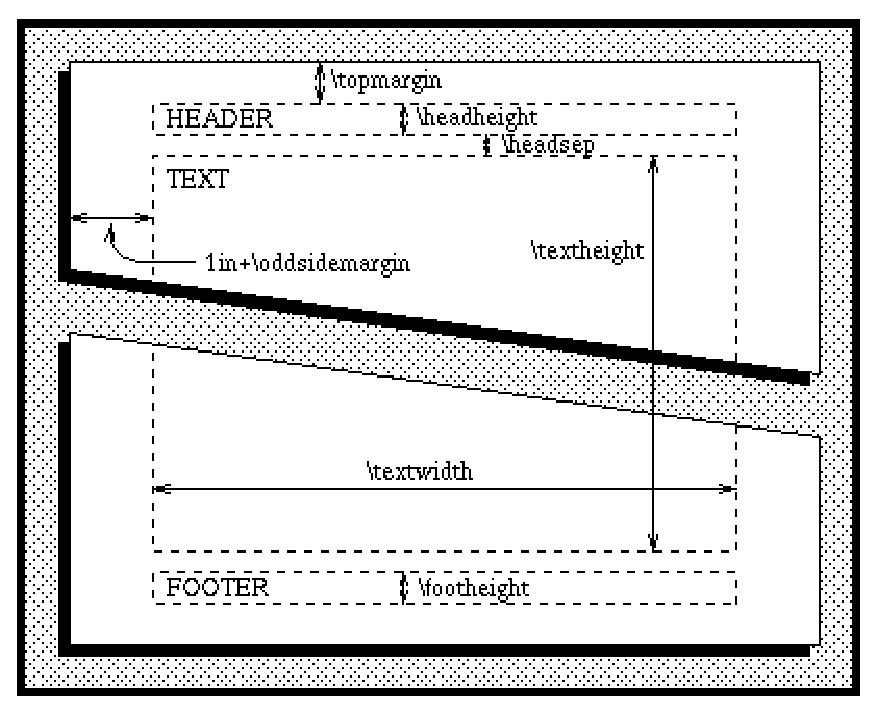
\epsfig{file=pagesetup.eps,scale=.65}\footnote{Image courtesy of Peter Newbury.}
%This slide was rather difficult. One major problem was Photoshop did not use correct headers in the EPS file. Nevertheless, the .65 scale is a balance between image quality and showing the footnote. Any smaller then the image could not be read. Any larger then the footnote would be truncated. Using caution when editing this slide.
\end{slide}
%================================Slide 14
\begin{slide}{Margins (con't)}
\begin{itemize}
	\item Lengths can be set with, for example, \texttt{$\backslash$textheight 8.0in}.
	\item Practically, it is easier to add to the current length if you need more space.
	\item More length can be allocated with, for example, \texttt{$\backslash$addtolength\{$\backslash$textwidth\}\{2in\}}.
\end{itemize}
\end{slide}
%================================Slide 15
\begin{slide}{Margins (con't)}
	\begin{itemize}
		\item Optimally, students should use 1 inch margins, which is a pain to configure by hand.
		\item I suggest using the \texttt{fullpage} package with the following syntax:
			\begin{center}
				\texttt{$\backslash$usepackage[\textit{options}]\{fullpage\}}
			\end{center}
		\item I suggest looking at the \texttt{fullpage} documentations that is listed under ``Supplemental Documents'' on the website.
	\end{itemize}
\end{slide}
%================================Slide 16
\begin{slide}{Headers}
	\begin{itemize}
		\item I suggest using the \texttt{$\backslash$fancyhdr} package.
		\item After invoking the package, follow it with these commands:
			\begin{center}
				\texttt{$\backslash$pagestyle\{fancy\}}
			\end{center}
		\item \texttt{$\backslash$lhead\{\textit{text}\}}, \texttt{$\backslash$chead\{\textit{text}\}}, and \texttt{$\backslash$rhead\{\textit{text}\}} will place text justified on the left, center, and right, respectively.
	\end{itemize}
\end{slide}
%================================Slide 17
\begin{slide}{Headers (con't)}
	\begin{itemize}
		\item By default, the left header will be the section number and section title of the page you are currently reading.
		\item If you do not want any header in the upper left, but a header in the upper right, then use:
			\begin{center}
				\texttt{$\backslash$lhead\{\}} \\
				\texttt{$\backslash$rhead\{\textit{text}\}}
			\end{center}
	\end{itemize}
\end{slide}
%================================Slide 18
\begin{slide}{Headers (con't)}
	\begin{itemize}
		\item If you are using a two--sided document, even and odd pages can be differentiated using:
			\begin{center}
				\texttt{$\backslash$lhead{}} \\
				\texttt{$\backslash$fancyhead[\textit{position}]\{\textit{text}\}}
			\end{center}
		\item The \textit{position} is where the position and page is defined.
	\end{itemize}
\end{slide}
%================================Slide 19
\begin{slide}{Headers (con't)}
	\begin{center}
	\begin{tabular}{l l||l l}
		\hline
		R & Right Side & E & Even Pages \\
		L & Left Side	 & O & Odd Pages \\
		C & Center		 &	 & \\
		\hline
	\end{tabular}
	\end{center}
	\begin{itemize}
		\item For instance, RE places the text on the right side of even pages.
		\item Similarly, LO places the text on the left side of odd pages.
		\item If you are only using one--sided documents, all of the pages are considered odd numbered.
	\end{itemize}
\end{slide}
%================================Slide 20
\begin{slide}{Headers (con't)}
	\begin{itemize}
		\item Below is an example of different headers:
			\begin{center}
				\texttt{$\backslash$fancyhead[RE]\{\textit{text}\}} \\
				\texttt{$\backslash$fancyhead[LO]\{\textit{different text}\}}
			\end{center}
		\item To put the page number in center of the header, use:
			\begin{center}
				\texttt{$\backslash$fancyhf\{\}} \\
				\texttt{$\backslash$fancyhead[CO,CE]\{$\backslash$page\}}
			\end{center}		
	\end{itemize}
\end{slide}
%================================Slide 21
\begin{slide}{Review}
	\begin{itemize}
		\item \texttt{$\backslash$title}, \texttt{$\backslash$author}, and \texttt{$\backslash$institution} are available and are implemented with \texttt{$\backslash$maketitle}.
		\item Margins can be manually adjusted, but usually simply using the \texttt{fullpage} package will create a desired layout.
		\item \texttt{fancyhdr} has a lot of options, I suggest also reading the supplemental documents.
		\item Also, look at the notes for this lecture. I have included a trick so different headers for odd and even pages can be used without printing a double--sided document.
	\end{itemize}
\end{slide}


\end{document}
